\subsection{Wissensbasis}
Die Wissensbasis stellt den zentralen Teil eines Expertensystems \cite[S.754]{wachsmuth1993}. Allgemein werden bei der Entwicklung der Wissensbasis zwei Aspekte behaldelt, n�mlich den Inhalt der Wissensbasis und die Wissensrepr�sentation. Der Inhalt der Wissensbasis l�sst sich in folgende Arten von Wissen unterteilen \cite{beierle2014}[S.5]:
\begin{itemize}
\item \textit{Fachspezifisches Wissen}. Dabei handelt es sich um das spezifischste Wissen, das sich
nur auf den gerade betrachteten Problemfall bezieht. Das sind z.B. Fakten, die von Beobachtungen oder Untersuchungsergebnissen stammen.
\item \textit{Regelhaftes Wissen}, das den eigentlichen Kern der Wissensbasis darstellt. Dieses Wissen kann noch genauer differenziert werden: 
	\begin{itemize}
	\item \textit{Bereichsbezogenes Wissen}, das sich auf den gesamten Problembereich beziehen. Das kann sowohl theoretisches Fachwissen als auch Erfahrungswissen sein. Anders gesagt handelt es sich um generisches Wissen.
	\item \textit{Allgemeinwissen}, das z.B. um generelle Probleml�sungsheuristiken, Optimierungsregeln oder auch allgemeines Wissen �ber Objekte und Beziehungen in der realen Welt beinhaltet.
	\end{itemize}
\end{itemize}
Beierle und Kern-Isberner bieten in der Abbildung \ref{expertensystem_beierle} eine alternative Darstellung eines Expertensystems mit Ber�cksichtigung der verschiedenen Arten des Wissens:
\begin{figure}[H] 
	\centering
	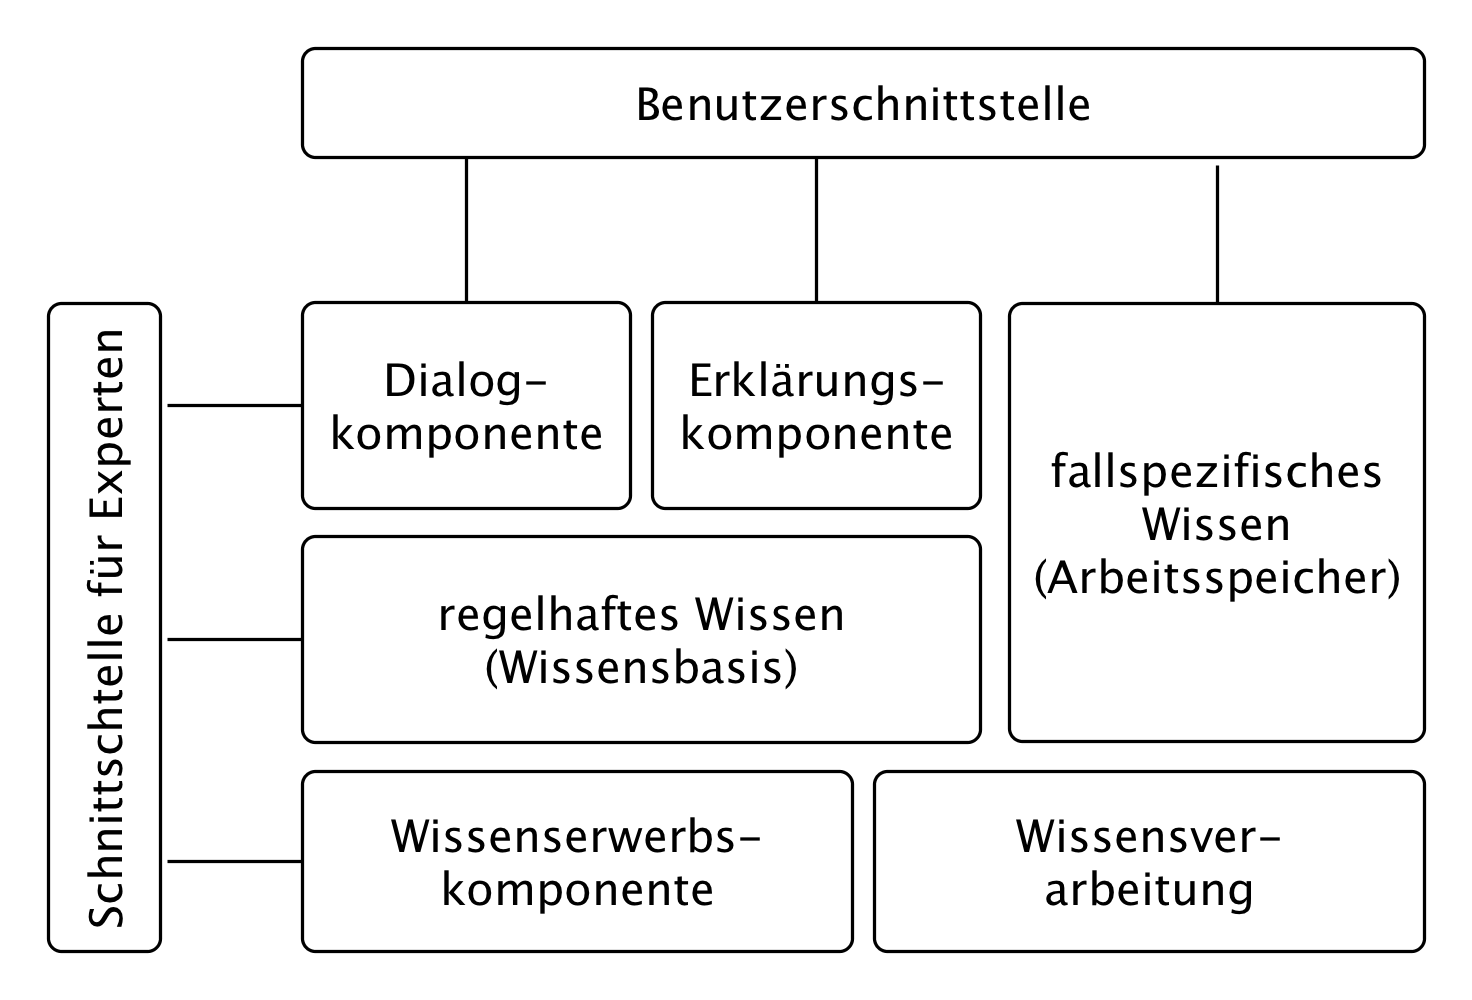
\includegraphics[width=0.75\textwidth]{images/expertensystem_beierle.png}
	\caption{Expertensystems nach Beierle und Kern-Isberner, \cite[S.18]{beierle2014}}
	\label{expertensystem_beierle}
\end{figure} 
Laut Beierle und Kern-Isberner k�nnen verschiedene Wissensarten in einem wissensbasierten System in sehr unterschiedlichem Umfang auftreten. Ein hochspezialisiertes System kann beispielsweise �ber sehr wenig oder gar kein Allgemeinwissen verf�gen. Auf der anderen Seite kann ein anderes System den Schwerpunkt auf das gew�hnliche Alltagswissen legen \cite[S.5-6]{beierle2014}.\\
Ein weiterer Aspekt beim Aufbau der Wissensbasis ist die Wissensrepr�sentation. Die grundlegende Aufgabe der Wissensrepr�sentation ist die Formularisierung von Wissen, um eine maschinelle Verarbeitung  erst zu erm�glichen \cite[S.22]{haun2000}. Sinz und Ferstl unterscheiden folgende Formen der Wissensrepr�sentation \cite[S.366]{sinz2013}:
\begin{itemize}
\item \textit{Regelorientierte Darstellung}, in der das Wissen als (WENN, DANN)-Beziehungen beschrieben wird. Diese Darstellungsform wird beispielsweise bei Prolog-Regeln eingesetzt.
\item \textit{Objektorientierte Darstellung}, die das Konzept der Objekttypen �bernimmt und mit deklarativen Operatorbeschreibungen verbindet.
\item \textit{Constraints Darstellung}, die Modellbeschreibungen aus dem Operations Research benutzt. Dabei handelt es sich um L�sungsr�ume durch Nebenbedingungen und Zielvorgaben.   
\end{itemize}
Hinsichtlich der Umsetzung der Wissensbasis stellen Ferstl und Sinz imperative und deklarative Paradigmen gegen�ber \cite[S.366]{sinz2013}. Ein Programm, das dem imperativen Paradigma folgt, besteht aus einer Folge von Befehlen, die nacheinander ausgef�hrt werden \cite[S.341]{sinz2013}. Bei einem deklarativen Programm handelt es sich um eine Beschreibung der Aufgabenau�ensicht. Ein deklaratives Programm hat keine festgelegten L�sungsverfahren je Aufgaben. Stattdessen wird eine L�sung zum Zeitpunkt der Aufgabendurchf�hrung mittels Inferenzmaschine abgeleitet \cite[S.361]{sinz2013}.\\
Allgemein beziehen sich die Autoren darauf, dass ein wissensbasiertes System nur geringe Anforderungen bez�glich Vollst�ndigkeit, Widerspruchsfreiheit und Eindeutigkeit gestellt werden k�nnen. Daher ist das deklarative Paradigma zu empfehlen. Folgende Gr�nde sprechen f�r die deklarative Umsetzung der Wissensbasis \cite[S.366]{sinz2013}: 
\begin{itemize}
\item \textit{Wissensdarstellung}: Da ein Mensch das Erfahrungswissen durch assoziative Beziehungsmuster aufbaut, ist die deklarative Wissensdarstellung eher geeignet.
\item \textit{Wissensauswertung}: �nderungen von Erfahrungswissen werden normalerweise in deklarativen Form erfasst.
\item \textit{Wissensverf�gbarkeit}: Die Codewartung von einem imperativen Programm ist fehleranf�llig, kosten- und zeitintensiv, da das Erfahrungswissen h�ufig ge�ndert und aktualisiert werden muss.
\end{itemize}
Der objektorientierte Ansatz ist eine weitere M�glichkeit, die Wissensbasis umzusetzen. Ein Beispiel f�r die objektorientierte Implementierung wird in \cite{leung1990} vorgestellt. Die Wissensbasis wird dabei als eine Sammlung von Klassen, Objekten und Methoden definiert \cite[S.40]{leung1990}. Der gro�e Vorteil solcher Umsetzung besteht in der Modularit�t des Wissens. Das Wissen in unabh�ngige Module aufgeteilt wird. Da die einzelnen Module unabh�ngig voneinander sind, k�nnen sie getrennt getestet und modifiziert werden, ohne den Rest der Wissensbasis zu beeintr�chtigen. Dies erm�glicht hohe Flexibilit�t bei der Wissensbasiserweiterung \cite[S.43]{leung1990}.\\
Neben der Implementierung der Wissensbasis ist eine geeignete Umsetzung der Wissensakquisitionskomponente erforderlich, um die Wissensbasis aktuell, m�glichst fehlerfrei und konsistent zu halten. Im Folgenden wird die Wissensakquisitionskomponente in Hinsicht auf den allgemeinen Aufbau und Funktionen thematisiert.  